\documentclass[12pt]{amsart}

% ------------------------------------------------------------------------------
% Packages
% ------------------------------------------------------------------------------
\usepackage[utf8]{inputenc} % input encoding
\usepackage{framed} % for \framebox
\usepackage[english]{babel} % language support 
\usepackage[colorlinks=true, linkcolor=blue, urlcolor=blue, citecolor=blue, anchorcolor=blue]{hyperref} % hyperref package
\usepackage{amsthm, amsmath, amsfonts, mathtools, amssymb, bm} % Math packages
\usepackage{xcolor} % Color package
\usepackage[shortlabels]{enumitem} % Enumeration package
\usepackage{booktabs}
\usepackage{float}
\usepackage{cancel}

% ------------------------------------------------------------------------------
% Document Style
% ------------------------------------------------------------------------------

% Header ----------------------------------------------------------------------
\addtolength{\hoffset}{-2.25cm}
\addtolength{\textwidth}{4.5cm}
\addtolength{\voffset}{-2.5cm}
\addtolength{\textheight}{5cm}
\setlength{\parskip}{0pt}
\setlength{\parindent}{15pt}

\pagestyle{myheadings}

\setlength{\parindent}{0in}

\pagestyle{empty}
\makeatletter
\def\fps@figure{H}
\def\fps@table{H}
% ------------------------------------------------------------------------------

% ------------------------------------------------------------------------------
% New commands
% ------------------------------------------------------------------------------
\newcommand{\qiq}{\qquad \implies \qquad}
\newcommand{\qiffq}{\qquad \iff \qquad}
\newcommand{\qaq}{\qquad \textbf{and} \qquad}
\newcommand{\qoq}{\qquad \textbf{or} \qquad}

% ------------------------------------------------------------------------------
% New environments
% ------------------------------------------------------------------------------
\newtheorem*{theorem}{\color{red!60!black}Theorem}
\newtheorem{corollary}{\color{blue}Corollary}
\counterwithin*{corollary}{subsection}
\newtheorem{lemma}{\color{blue}Lemma}
\counterwithin*{lemma}{subsection}
\newtheorem{proposition}{\color{blue}Proposition}
\counterwithin*{proposition}{subsection} 
\theoremstyle{definition}
\newtheorem*{definition}{\color{green!60!black}Definition}
\newtheorem{example}{\color{orange!80!black}Example}
\newtheorem*{Obs}{\color{purple!80!white}Observation}
\newtheorem*{As}{\color{red!80!white}Assumptions}
\newtheorem*{answer}{\color{red!60!white}Answer}
\newtheorem*{Cor}{\color{blue!60!white}Corollary}
\newtheorem{exercise}{\color{blue!60!white}Exercise}
\newtheorem{subexercise}{ \color{blue!40!white}  }[exercise]

\begin{document}

\thispagestyle{empty}


{\scshape FIN-971} \hfill {\scshape \Large Problem Set \#3} \hfill {\scshape Fall 2021}\\
{\scshape Author(s): \hfill Mitchell Valdes-Bobes\\
{\scshape Date: \hfill \texttt{12/12/21}
\medskip

\hrule

\bigskip

\bigskip
    
\begin{exercise}[ $3.15$ of Tirole (project riskiness and credit rationing).]
Consider the basic, fixed-investment model covered in Section $3.2$ of Tirole (2006). 
In particular, investment is a fixed size $I$, the entrepreneur borrows $I-A$, the probability of success is either $p_{H}$ (which
yields no private benefit) or $p_{L}$ (which yields private benefit $B$ ), success yields verifiable revenue $R$ while failure yields 0.
There are two types, "$A$" and "$B$", of the projects, which differ only with respect to "riskiness" defined by $p_{H}^{A} R^{A}=p_{H}^{B} R^{B}$,
but $p_{H}^{A}>p_{H}^{B}$ so that project $B$ is "riskier". The investment cost $I$ is the same for both variants and furthermore,
$\Delta p=p_{L}^{A}-p_{L}^{A}=p_{H}^{B}-p_{L}^{B}$. Which type of project is less prone to credit rationing?
\end{exercise}

\begin{answer}
    From the Second Best financing problem we have that the necessary condition for funding is that 
    $$
    \mathcal{P}_{0}^i  \equiv p^i_{H}\left(R^i-\frac{B}{\Delta p}\right) \geq I-A \qquad i\in\{A,B\}
    $$

    Note that $\mathcal{P}_{0}^A - \mathcal{P}_{0}^B =  (p^A_{H} - p^B_{H}) \left(R^i-\frac{B}{\Delta p}\right)> 0$. 

    From this, we can see that all other things being equal if a project of type $B$ gets funded then a project of type $A$ will also get funded, but the 
    the opposite is not necessarily true.
    Thus, the project of type $B$, the riskier one, is more prone to credit rationing.

\end{answer}

\begin{exercise}[$3.13$ of Tirole (lender market power with fixed investment).] 
The environment is similar to Section $3.2$ of Tirole with one exception. An entrepreneur has internal wealth $A$ (which could be
negative because of previous debt) and wants to undertake non-negative investment $I>A$ into a fixed-size project.
The project yields $R>0$ with probability $p$ and 0 with probability $1-p$. The probability of success is $p_{H}$ if the entrepreneur
works and $p_{L}<p_{H}$ if he shirks. The entrepreneur obtains private benefit $B$ if she shirks and 0 otherwise. The borrower is
protected by limited liability and everyone is risk-neutral. The project is worthwhile only if the entrepreneur behaves.

The exception is that there is a single lender. This lender has access to funds that command an expected rate of return equal to 0
(so the lender would content himself with a 0 rate of return, but will use his market power to obtain a superior rate of return).
Assume $V \equiv$ $p_{H} R-I>0$ and let $\bar{A}$ and $\widehat{A}$ be defined by
$$
\begin{aligned}
\bar{A} & \equiv I-p_{H}\left[R-\frac{B}{\Delta p}\right] \\
\widehat{A} & \equiv p_{H} \frac{B}{\Delta p}
\end{aligned}
$$
where $\Delta p=p_{H}-p_{L}$. Assume that $\bar{A}>0$ and that the lender makes a take-it-or-leave-it offer to the borrower (i.e.the lender chooses $R_{b}$, the borrower's compensation in the case of success).

\end{exercise}
\begin{subexercise}
    What contract is optimal for the lender? Be sure to state the programming problem explicitly.
\end{subexercise}
\begin{answer}
    The lender maximizes their profits subject to $IC$ and participation constraints for the borrower holds:
    
    \begin{align*}
        \max _{R_{l}, R_{b}} &p_{H} R_{l}-I+A & \\
        \text { s.t. } p_{H} R_{b} & \geq p_{L} R_{b}+B \\
        p_{H} R_{b} & \geq A \\
        p_{H} R_{l} & \geq I-A \\
        R_{l}+R_{b} & =R \\
    \end{align*}
    

    Thus, the lender will choose the lowest $R_{b}$ such that all constraints hold. First let $\hat{A}$ be the net worth where $I C_{b}$ and $P C_{b}$ both bind:
    $$
    \frac{B}{\Delta p}=\frac{\hat{A}}{p_{H}} \Longrightarrow \hat{A}=p_{H} \frac{B}{\Delta p}
    $$
    Second, observe that the $P C_{b}$ and $P C_{l}$ cannot both bind. Suppose not then
    $$
    \frac{A}{p_{H}}=R-\frac{I-A}{p_{H}} \Longrightarrow 0=p_{H} R-I=V>0 \Rightarrow \Leftarrow
    $$
    Third, let $\bar{A}$ be the net worth where the $I C_{b}$ and $P C_{l}$ both bind:
    $$
    \frac{B}{\Delta p}=R-\frac{I-\bar{A}}{p_{H}} \Longrightarrow \bar{A}=I-p_{H}\left(R+\frac{B}{\Delta p}\right)
    $$
    Thus, the optimal lending contract for the lender depends on $A .$ If $A<\bar{A}$, then the lenders participation constraint does not hold, so there's no contract (i.e. credit rationing). If $\bar{A} \leq A<\hat{A}$, the borrowers incentive compatibility constraint binds and the borrowers participation constraint is slack, so $R_{b}=\frac{B}{\Delta p} .$ At $A=\hat{A}$, both the borrowers incentive compatibility and participation constraints bind. If $I>A>\hat{A}$, the borrowers incentive compatibility constraint is slack and the borrowers participation constraint binds, so $R_{b}=\frac{A}{p_{H}}$.
\end{answer}

\begin{subexercise}
    Is the financing decision affected by lender market power (i.e. compared to the case of competitive lenders in Section 3.2)?

\end{subexercise}

\begin{answer}
    Lender market power does not affect the financing decision.
\end{answer}

\begin{subexercise}
    Draw the borrower's net utility (i.e. net of $A$ ) as a function of $A$. Note that unlike the monotonic case in Section 3.2,
    it is nonmonotonic among the regions $(-\infty, \bar{A}),[\bar{A}, \widehat{A}),[\widehat{A}, I)$. Explain.
\end{subexercise}

\begin{answer}
    The borrower's net utility is:
    \begin{center}
        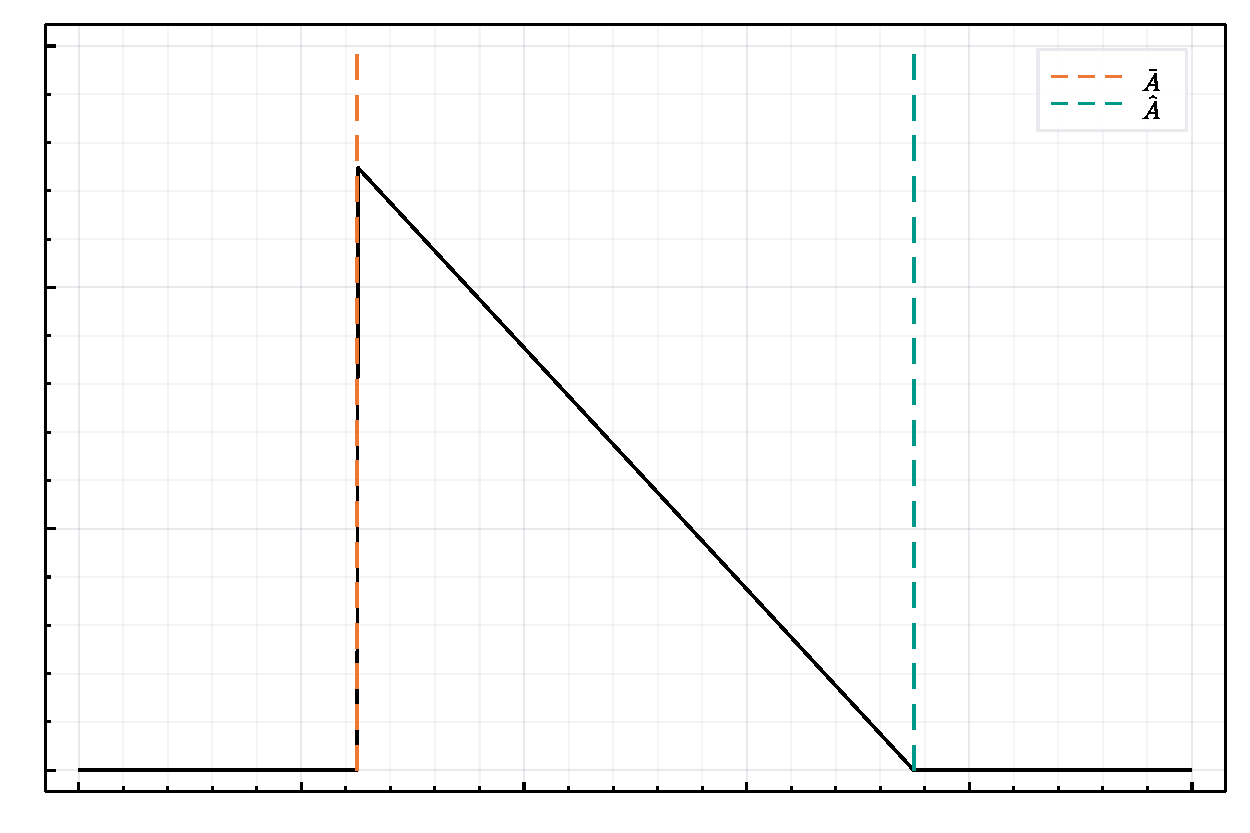
\includegraphics[width=0.5\textwidth]{figures/exercise_2_1.pdf}
    \end{center}
\end{answer}

\begin{exercise}[$3.5$ of Tirole (continuous investment and decreasing returns to scale).]
    Consider the continuous investment model of Section $3.4$ of Tirole (2006) with one modification; investment $I$ yields return $R(I)$ 
    in the case of success and 0 in the case of failure, where $R^{\prime}>0$ and $R^{\prime \prime}<0, R^{\prime}(0)>1 / p_{H}, R^{\prime}(\infty)<1 / p_{H}$. 
    The rest of the model is unchanged. That is, the entrepreneur starts with cash $A$, the probability of success is either $p_{H}$ if he behaves or $p_{L}$ 
    if he misbehaves. The entrepreneur obtains private benefit $B I$ if he misbehaves and 0 otherwise. Only the final outcome is observable. Let $I^{*}$ 
    denote the level of investment that maximizes total surplus (i.e. $p_{H} R^{\prime}\left(I^{*}\right)=1$ ).
\end{exercise}

\begin{subexercise}
    How does investment $I(A)$ vary with the level of cash?
\end{subexercise}

\begin{answer}
    The problem is

\begin{align*}
    \max _{I, R_{b}} &\quad p_{H} R_{b} \\
    \text { s.t. } &\quad R_{b}  \geq \frac{B I}{\Delta p} \qquad \left(I C_{b}\right) \\
                    &\quad  R_{b} \leq R(I)-\frac{I-A}{p_{H}} \qquad {\left(P C_{l}\right)}
\end{align*}

$P C_{l}$ binds.if not then $R_{b}$ can be increased without violating any constraint which increases the objective function.
$$
R_{b}=R(I)-\frac{I-A}{p_{H}}
$$
Differentiating with respect to $I$, we get:
$$
\frac{d R_{b}}{d I}=R^{\prime}(I)-\frac{1}{p_{H}}
$$

$R^{\prime}(I), R_{b}$ is increasing in $I$ for all $I<I^{*}$. So the borrower would choose the highest $I$ as possible. Thus, $I C_{b}$ binds for all $I \leq I^{*}$. Suppose not, then the borrower would go to a different lender. Taking $I C_{b}$ and $P C_{l}$ together:
$$
R(I)-\frac{I-A}{p_{H}}=\frac{B I}{\Delta p}
$$
This holds  at $I^{*} .$ By total differentiation and  $R^{\prime}\left(I^{*}\right)-\frac{1}{p_{H}}=0$,
$$
R^{\prime}\left(I^{*}\right) d I-\frac{d I-d A}{p_{H}}=\frac{B d I}{\Delta p} \Longrightarrow\left[R^{\prime}\left(I^{*}\right)-\frac{1}{p_{H}}\right] d I+\frac{d A}{p_{H}}=\frac{B d I}{\Delta p} \Longrightarrow \frac{d I}{d A}=\frac{\Delta p}{B p_{H}}>0
$$
So $I$ is increasing in $A$ since all terms in the above expression are positive.
\end{answer}

\begin{subexercise}
    How does the shadow value $v$ of cash (the derivative of the borrower's gross utility with respect to cash) vary with the level of cash?
\end{subexercise}

\begin{answer}

\end{answer}

\end{document}